\documentclass[12pt,a4paper,titlepage]{article}
\usepackage[utf8]{inputenc}
\usepackage{amsmath}
\usepackage{algorithm}
\usepackage[noend]{algpseudocode}
\usepackage{amsfonts}
\usepackage{amssymb}
\usepackage{graphicx}
\usepackage{color}
\usepackage[margin=1in]{geometry}
\author{800107 - Daniel Ng See Cheong\\
		839521 - Uzair Moolla}
\title{
	AAA Project\\
	\large Solving Sudoku using the backtracking algorithm
}

\graphicspath{ {images/} }

\newcommand{\todo}[1]{\textcolor{red}{\textbf{\##1\#}}}

\begin{document}
\maketitle

\section{Introduction}
Sudoku is a numerical based logic puzzle game. The idea is to fill in an $n\times n$ grid with numbers in a specific manner. The most commonly known grid usually consists of square blocks with 3 rows and 3 columns. These individual blocks are then arranged in a similar manner again, with 3 blocks along rows and 3 along columns, producing a $9 \times 9$ matrix. An example of this described matrix can be seen in Figure  \ref{fig:Blank_Sudoku_Board}. We need to fill each of the blocks with one of these numbers ${1,2,3,4,5,6,7,8,9}$. The rules for filling these blocks are as follows:
\begin{itemize}
\item[•] Within each $3 \times 3 $ block we can only have single occurrence of each number.
\item[•] Along each $9$ block row we can only have a single occurrence of each number.
\item[•] Along each $9$ block column we can only have a single occurrence of each number.
\end{itemize}

\noindent
An example of a Sudoku Puzzle completed using the rules stated above can be seen in Figure \ref{fig:Complete_Sudoku_Board}.

\begin{figure}[h]
\centering
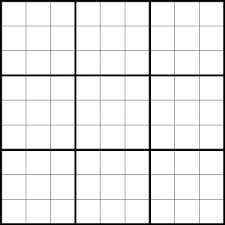
\includegraphics[scale=0.5]{Blank_Sudoku_Board}
\caption{Sample of a $9\times9$ Blank Sudoku Board}
\label{fig:Blank_Sudoku_Board}
\end{figure}
%-------------------------------------------------------%
\begin{figure}[h]
\centering
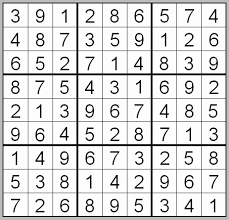
\includegraphics[scale=0.5]{Complete_Sudoku_Board}
\caption{Sample of a $9\times9$ Completed Sudoku Board}
\label{fig:Complete_Sudoku_Board}
\end{figure}
%------------------------------------------------------%

\noindent
Solving sudoku puzzles are a fun exercise for many. However we would like to find a suitable algorithm which can be used to solve sudoku puzzles correctly as well as efficiently. There are various possible methods which can be used to solve sudoku puzzles. We will be focussing on the \emph{Backtracking Algorithm} in our experiments.
\\
\todo{Fill in facts}

\newpage
\section{Aims}

We are going to use the backtracking algorithm to solve sudoku puzzles of size $n\times n$. We will attempt to solve these sudoku
puzzles in as little time as possible. Once we have the algorithm working correctly we will perform both empirical as well as
theoretical analysis on it. We aim to find the best, average and worst case complexities of the algorithm being used.
\\
\todo{add some stuff}

\section{Summary of Theory}

\section{Pseudo code}
\begin{algorithm}
\caption{Backtracking}
\begin{algorithmic}
\Function{name}{params}
  \If{\textit{empty}} 
  \State \todo{fill in}
  \Else
  \State continue
  \EndIf
  \State \Return something
\EndFunction
\end{algorithmic}
\end{algorithm}

\section{Experimental Methodology}

\section{Presentation of results}

\section{Interpretation of results}

\section{Conclusion}

\section{References}

\section{Acknowledgements}

\end{document}